%
% File udst2018.tex

\documentclass[11pt,a4paper]{article}
\usepackage[T1]{fontenc}
\usepackage[hyperref]{udst2018}
\usepackage{times}
\usepackage{latexsym}
\usepackage{amsmath}
\usepackage{tikz}
\usepackage{tikz-dependency}
\usepackage[warn]{textcomp}
\usepackage[font=small]{caption}
\usepackage{subcaption}
\usepackage{multirow}
\usepackage{url}
\usepackage{etoolbox}
\usepackage{xr}
\usepackage{adjustbox}
\usepackage{pgfplots,pgfplotstable}

\newcommand{\com}[1]{}
\newcommand{\oa}[1]{\footnote{\color{red}OA: #1}}
\newcommand{\daniel}[1]{\footnote{\color{blue}Daniel: #1}}

\DeclareMathOperator*{\argmin}{argmin}
\DeclareMathOperator*{\argmax}{argmax}

\makeatletter
\patchcmd\@combinedblfloats{\box\@outputbox}{\unvbox\@outputbox}{}{%
   \errmessage{\noexpand\@combinedblfloats could not be patched}%
}%
 \makeatother


\hyphenation{UDPipe}

\usetikzlibrary{shapes,shapes.misc}


\aclfinalcopy 
\def\aclpaperid{8} %  Enter the Paper ID here for final camera ready copy

%\setlength\titlebox{5cm}
% You can expand the titlebox if you need extra space
% to show all the authors. Please do not make the titlebox
% smaller than 5cm (the original size); we will check this
% in the camera-ready version and ask you to change it back.

\title{Universal Dependency Parsing with a \\ General Transition-Based DAG Parser}

\author{Daniel Hershcovich$^{1,2}$ \\
  \\\And
  Omri Abend$^2$ \\
  $^1$The Edmond and Lily Safra Center for Brain Sciences \\
  $^2$School of Computer Science and Engineering \\
  Hebrew University of Jerusalem \\
  \texttt{\{danielh,oabend,arir\}@cs.huji.ac.il}
  \\\And
  Ari Rappoport$^2$
}

\date{}

\begin{document}
\maketitle
\begin{abstract}
  We apply TUPA, a neural transition-based general DAG parser,
  as the submission by the HUJI team to the CoNLL 2018 UD shared task.
  TUPA was designed for parsing UCCA, a cross-linguistic
  semantic annotation scheme, exhibiting
  reentrancy, discontinuity and non-terminal nodes.
  By employing a conversion protocol to represent
  UD trees and graphs in a UCCA-like unified directed acyclic graph (DAG) format,
  we train TUPA almost without modification on the UD parsing task.
  Although not among the leading submissions in the task,
  the results are promising given the uniform parsing architecture,
  which allows recovering enhanced relations and shared arguments,
  as well as multitask learning.
  Our code is available at \url{https://github.com/CoNLL-UD-2018/HUJI}.
\end{abstract}

\section{Introduction}\label{sec:introduction}

In this paper we describe the HUJI submission to the CoNLL 2018 shared task
on Universal Dependency parsing \cite{udst:overview2018}.
We focus only on parsing, using a baseline model \cite[UDPipe 1.2;][]{udpipe,udpipe:2017}
for tokenization, sentence splitting, part-of-speech tagging and morphological tagging.
Our system is based on TUPA \cite[see \S\ref{sec:model}]{hershcovich2017a,hershcovich2018multitask},
a transition-based UCCA parser.
UCCA \cite[Universal Conceptual Cognitive Annotation;][]{abend2013universal} is a
cross-linguistic semantic annotation scheme, representing scenes, participants,
attributes and relations in a directed acyclic graph (DAG) structure,
and allowing reentrancy (argument sharing),
discontinuity (corresponding to non-projectivity in dependency annotations)
and non-terminal nodes (as opposed to dependencies, which are bi-lexical).
To parse Universal Dependencies \cite{nivre2016universal}
using TUPA, we employ a conversion protocol to represent
UD trees and graphs in a UCCA-like unified DAG format (\S\ref{sec:format}).

\begin{figure}[ht]
\fbox{\begin{subfigure}{0.47\textwidth}
    \centering
    \scalebox{.95}{
    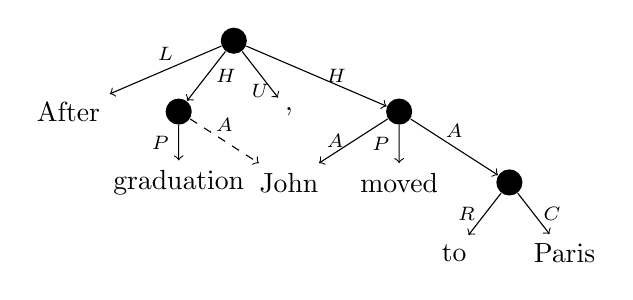
\begin{tikzpicture}[level distance=9mm, sibling distance=14mm, ->,
        every circle node/.append style={fill=black}]
      \tikzstyle{word} = [font=\rmfamily,color=black]
      \node (ROOT) [circle] {}
        child {node (After) [word] {After} edge from parent node[above] {\scriptsize $L$}}
        child {node (graduation) [circle] {}
        {
          child {node [word] {graduation} edge from parent node[left] {\scriptsize $P$}}
        } edge from parent node[right] {\scriptsize $H$} }
        child {node [word] {,} edge from parent node[below] {\scriptsize $U$}}
        child {node (moved) [circle] {}
        {
          child {node (John) [word] {John} edge from parent node[left] {\scriptsize $A$}}
          child {node [word] {moved} edge from parent node[left] {\scriptsize $P$}}
          child {node [circle] {}
          {
            child {node [word] {to} edge from parent node[left] {\scriptsize $R$}}
            child {node [word] {Paris} edge from parent node[right] {\scriptsize $C$}}
          } edge from parent node[above] {\scriptsize $A$} }
        } edge from parent node[right] {\scriptsize $H$} }
        ;
      \draw[dashed,->] (graduation) to node [above] {\scriptsize $A$} (John);
    \end{tikzpicture}}
  \caption{Example UCCA graph.}
  \label{fig:converted_example_ucca}
\end{subfigure}}
\fbox{\begin{subfigure}{0.47\textwidth}
  \centering
    \begin{dependency}[text only label, label style={above}, font=\small]
    \begin{deptext}[column sep=.8em,ampersand replacement=\^]
    After \^ graduation \^ , \^ John \^ moved \^ to \^ Paris \\
    \end{deptext}
        \depedge{2}{1}{case}
        \depedge{4}{3}{punct}
        \depedge{5}{4}{nsubj}
        \depedge[edge end x offset=-2pt]{2}{5}{obl}
        \depedge{7}{6}{case}
        \deproot[edge unit distance=3ex]{5}{root}
        \depedge[edge unit distance=3ex]{5}{7}{obl}
    \end{dependency}
  \caption{\label{fig:original_examples}Example UD tree.}
\end{subfigure}}
\fbox{\begin{subfigure}{0.47\textwidth}
  \centering
  \scalebox{.95}{
  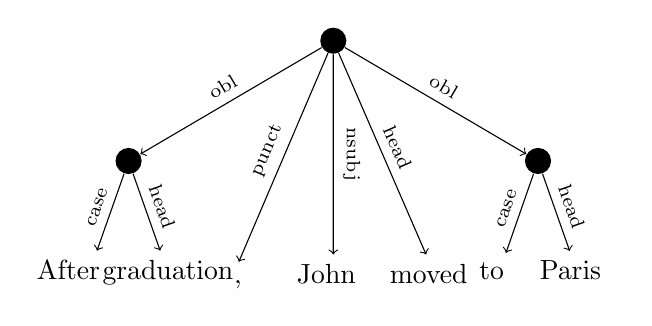
\begin{tikzpicture}[level distance=17mm, ->,
      every node/.append style={sloped,anchor=south,auto=false,font=\scriptsize},
      level 1/.style={sibling distance=13mm},
      level 2/.style={sibling distance=1cm}]
    \tikzstyle{word} = [font=\rmfamily,color=black]
    \node (ROOT) [fill=black,circle] {}
      child {node (after) [fill=black,circle] {}
      {
        child {node [word] {After{\color{white}g}\quad\quad} edge from parent node {case}}
        child {node [word] {\quad graduation\quad\quad} edge from parent node {head}}
      } edge from parent node {obl}}
      child {node {}
      {
        child {node [word] (comma) {\quad,{\color{white}g}} edge from parent [draw=none]}
      } edge from parent [draw=none]}
      child {node {}
      {
        child {node [word] (John) {John{\color{white}g}} edge from parent [draw=none]}
      } edge from parent [draw=none]}
      child {node {}
      {
        child {node [word] (moved) {moved{\color{white}g}} edge from parent [draw=none]}
      } edge from parent [draw=none]}
      child {node (to) [fill=black,circle] {}
      {
          child {node [word] {to{\color{white}g}} edge from parent node {case}}
          child {node [word] {Paris{\color{white}g}} edge from parent node {head}}
      } edge from parent node {obl}}
      ;
      \draw (ROOT) to node {punct} (comma);
      \draw (ROOT) to node {nsubj} (John);
      \draw (ROOT) to node {head} (moved);
  \end{tikzpicture}}
  \captionof{figure}{UD tree after conversion to unified DAG format.}\label{fig:converted_example_ud}
\end{subfigure}}

\caption{(a) Example UCCA annotation for the sentence
``After graduation, John moved to Paris''.
The dashed \textit{A} edge is a \textit{remote edge},
representing a \textit{Participant} relation that is not explicit in the text,
and allowing argument sharing and reentrancy,
creating a DAG structure.
(b) Bilexical tree annotating the same sentence according to the UD guidelines.
(c) The same UD tree, after conversion to the unified DAG format.
Intermediate non-terminals and \textit{head} edges are introduced,
to get a UCCA-like structure.}\label{fig:converted_examples}
\end{figure}


%%%%%%%%%%%%%%%%%%%%%%%%%%%%%%%%%%%%%%%%%%%%%%%%%%%%%%%%%%%%%%%%%%%%%%%%%%%%%%%%%%%%%%%%
\section{Unified DAG Format}\label{sec:format}

To apply TUPA to UD parsing,
we convert UD trees and graphs into a unified DAG format \cite{hershcovich2018multitask}.
The format consists of a rooted DAG, where the tokens are the terminal
nodes.\footnote{Our conversion code supports full conversion between UCCA and UD,
among other representation schemes,
and is publicly available at \url{http://github.com/danielhers/semstr/tree/master/semstr/conversion}.}
As in the UCCA format, edges are labeled (but not nodes),
and are divided into \textit{primary} and \textit{remote} edges,
where the primary edges form a tree (all nodes have at most one primary parent,
and the root has none).
Remote edges enable reentrancy, and thus together with primary edges
form a DAG.
Figure~\ref{fig:converted_examples} shows an example a UCCA graph,
and a UD tree before and after conversion.

To convert UD into the unified DAG format,
we add a pre-terminal for each token,
and attach the pre-terminals according to the original dependency edges:
traversing the tree from the root down, for each head token we create a non-terminal
parent with the edge label {\it head},
and add the node's dependents as children of the created non-terminal node
(see Figure~\ref{fig:converted_example_ud}).
This creates a constituency-like structure,
which is supported by TUPA's transition set (see \S\ref{sec:transition_set}).

Any \textit{enhanced UD}\footnote{\url{http://universaldependencies.org/u/overview/enhanced-syntax.html}}
heads beyond the normal head of a node are converted to remote edges in the unified DAG format.
Although not included in the evaluation metrics for UD parsing,
we believe these enhancements, representing elided predicates,
shared arguments due to conjunction, control, raising and coreference,
case information,
as well as partitives and light noun constructions \cite{SCHUSTER16.779},
provide richer information to the parser, and may possibly even improve parsing performance
on the main dependency tree.

In the conversion process, we strip any language-specific relation subtypes
(ignored by the evaluation),
leaving only the universal relations:
for example, the language-specific \verb|acl:relcl| is replaced by the universal relation \verb|acl|.


%%%%%%%%%%%%%%%%%%%%%%%%%%%%%%%%%%%%%%%%%%%%%%%%%%%%%%%%%%%%%%%
\section{General Transition-based DAG Parser}\label{sec:model}

We now turn to describing TUPA \cite{hershcovich2017a,hershcovich2018multitask},
a general transition-based parser \cite{Nivre03anefficient}.
TUPA uses an extended set of transitions and features that supports
reentrancies, discontinuities and non-terminal nodes.
The parser state is composed of a buffer $B$ of tokens and nodes to be processed,
a stack $S$ of nodes currently being processed,
and a graph $G=(V,E,\ell)$ of constructed nodes and edges,
where $V$ is the set of \emph{nodes}, $E$ is the set of \emph{edges},
and $\ell : E \to L$ is the \emph{label} function, $L$ being the set of possible labels.
Some states are marked as \textit{terminal}, meaning that $G$ is the final output.
A classifier is used at each step to select the next transition based on features
encoding the parser's current state.
During training, an oracle creates training instances for the classifier,
based on gold-standard annotations.

\begin{figure*}
	\begin{adjustbox}{width=\textwidth,margin=3pt,frame}
	\begin{tabular}{llll|l|llllc|c}
		\multicolumn{4}{c|}{\textbf{\small Before Transition}} & \textbf{\small Transition} & \multicolumn{5}{c|}{\textbf{\small After Transition}} & \textbf{\small Condition} \\
		\textbf{\footnotesize Stack} & \textbf{\footnotesize Buffer} & \textbf{\footnotesize Nodes} & \textbf{\footnotesize Edges} & & \textbf{\footnotesize Stack} & \textbf{\footnotesize Buffer} & \textbf{\footnotesize Nodes} & \textbf{\footnotesize Edges} & \textbf{\footnotesize Terminal?} & \\
		$S$ & $x \;|\; B$ & $V$ & $E$ & \textsc{Shift} & $S \;|\; x$ & $B$ & $V$ & $E$ & $-$ & \\
		$S \;|\; x$ & $B$ & $V$ & $E$ & \textsc{Reduce} & $S$ & $B$ & $V$ & $E$ & $-$ & \\
		$S \;|\; x$ & $B$ & $V$ & $E$ & \textsc{Node$_X$} & $S \;|\; x$ & $y \;|\; B$ & $V \cup \{ y \}$ & $E \cup \{ (y,x)_X \}$ & $-$ &
		$x \neq \mathrm{root}$ \\
		$S \;|\; y,x$ & $B$ & $V$ & $E$ & \textsc{Left-Edge$_X$} & $S \;|\; y,x$ & $B$ & $V$ & $E \cup \{ (x,y)_X \}$ & $-$ &
		\multirow{4}{50pt}{\vspace{-5mm}\[\left\{\begin{array}{l}
		x \not\in w_{1:n},\\
		y \neq \mathrm{root},\\
		y \not\leadsto_G x
		\end{array}\right.\]} \\
		$S \;|\; x,y$ & $B$ & $V$ & $E$ & \textsc{Right-Edge$_X$} & $S \;|\; x,y$ & $B$ & $V$ & $E \cup \{ (x,y)_X \}$ & $-$ & \\
		$S \;|\; y,x$ & $B$ & $V$ & $E$ & \textsc{Left-Remote$_X$} & $S \;|\; y,x$ & $B$ & $V$ & $E \cup \{ (x,y)_X^* \}$ & $-$ & \\
		$S \;|\; x,y$ & $B$ & $V$ & $E$ & \textsc{Right-Remote$_X$} & $S \;|\; x,y$ & $B$ & $V$ & $E \cup \{ (x,y)_X^* \}$ & $-$ & \\
		$S \;|\; x,y$ & $B$ & $V$ & $E$ & \textsc{Swap} & $S \;|\; y$ & $x \;|\; B$ & $V$ & $E$ & $-$ &
		$\mathrm{i}(x) < \mathrm{i}(y)$ \\
		$[\mathrm{root}]$ & $\emptyset$ & $V$ & $E$ & \textsc{Finish} & $\emptyset$ & $\emptyset$ & $V$ & $E$ & $+$ & \\
	\end{tabular}
	\end{adjustbox}
	\caption{\label{fig:transitions}
	  The transition set of TUPA.
	  We write the stack with its top to the right and the buffer with its head to the left.
	  $(\cdot,\cdot)_X$ denotes a primary $X$-labeled edge, and $(\cdot,\cdot)_X^*$ a remote $X$-labeled edge.
	  $\mathrm{i}(x)$ is the swap index (see \S\ref{sec:constraints}).
	  In addition to the specified conditions,
	  the prospective child in an \textsc{Edge} transition must not already have a primary parent.
	}
\end{figure*}

\subsection{Transition Set}\label{sec:transition_set}
Given a sequence of tokens $w_1, \ldots, w_n$,
we predict a rooted graph $G$ whose terminals are the tokens.
Parsing starts with the root node on the stack,
and the input tokens in the buffer.

The TUPA transition set, shown in Figure~\ref{fig:transitions}, includes
the standard \textsc{Shift} and \textsc{Reduce} operations,
\textsc{Node$_X$} for creating a new non-terminal node and an $X$-labeled edge,
\textsc{Left-Edge$_X$} and \textsc{Right-Edge$_X$} to create a new primary $X$-labeled edge,
\textsc{Left-Remote$_X$} and \textsc{Right-Remote$_X$} to create a new remote $X$-labeled edge,
\textsc{Swap} to handle discontinuous nodes,
and \textsc{Finish} to mark the state as terminal.

Although the \textsc{Remote$_X$} transitions are not required for parsing trees,
we treat the problem as general DAG parsing, due to the inclusion of enhanced UD arcs
in the converted DAG format (see~\S\ref{sec:format}).


\begin{figure}[t]
   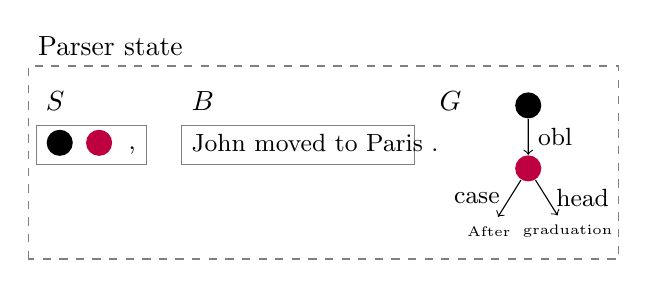
\begin{tikzpicture}[level distance=8mm, sibling distance=1cm]
   \node[anchor=west] at (0,1.5) {Parser state};
   \draw[color=gray,dashed] (0,-1.2) rectangle (7.5,1.25);
   \draw[color=gray] (.1,0) rectangle (1.5,.5);
   \node[anchor=west] at (.1,.8) {$S$};
   \node[fill=black, circle] at (.4,.275) {};
   \node[fill=purple, circle] at (.9,.275) {};
   \node[anchor=west] at (1.15,.175) {\small ,};
   \draw[color=gray] (1.95,0) rectangle (4.9,.5);
   \node[anchor=west] at (1.95,.8) {$B$};
   \node[anchor=west] at (1.95,.275) {\small John moved to Paris .};
   \node[anchor=west] at (5.1,.8) {$G$};
   \node[fill=black, circle] at (6.35,.75) {}
     child {node [fill=purple, circle] {}
     {
       child {node  {\tiny After} edge from parent [->] node[left] {\small case}}
       child {node {\tiny graduation} edge from parent [->] node[right] {\small head}}
     } edge from parent [->] node[right] {\small obl} };
   \end{tikzpicture}
   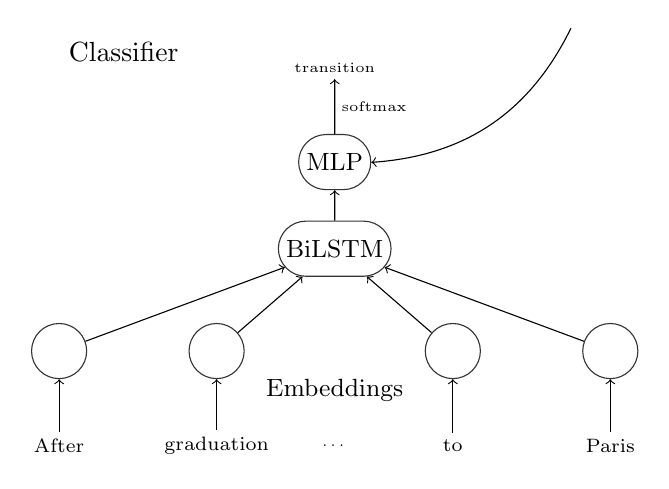
\begin{tikzpicture}[->]
   \node[anchor=west] at (0,6) {Classifier};
   \tiny
   \tikzstyle{main}=[rounded rectangle, minimum size=7mm, draw=black!80, node distance=12mm]
   \node[main] (specific) at (3.5,3.5) {\small BiLSTM};
   \node (embeddings) at (3.5,1.7) {\small Embeddings};
   \foreach \i/\word in {0/{After},2/{graduation},5/{to},7/{Paris}} {
       \node (x\i) at (\i,1) {\scriptsize \word};
       \node[main] (e\i) at (\i,2.2) {};
       \path (x\i) edge (e\i);
       \path (e\i) edge (specific);
   }
    \node (x4) at (3.5,1) {\ldots};
    \node[main] (mlp) at (3.5,4.6) {\small MLP};
    \path (specific) edge (mlp);
    \coordinate (state) at (6.5,6.3);
    \path (state) edge [bend left] (mlp);
    \node (transition) at (3.5,5.8) {transition};
    \path (mlp) edge node[right] {softmax} (transition);
   \end{tikzpicture}
\caption{Illustration of the TUPA model, from \citet{hershcovich2018multitask}.
Top: parser state (stack, buffer and intermediate graph).
		Bottom: BiLTSM architecture.
		Vector representation for the input tokens is computed
		by two layers of bidirectional LSTMs.
		The vectors for specific tokens are concatenated with
		embedding and numeric features from the parser state
		(for existing edge labels, number of children, etc.),
		and fed into the MLP for selecting the next transition.}\label{fig:single_model}
\end{figure}


%%%%%%%%%%%%%%%%%%%%%%%%%%%%%%%%%%%%%%%%%%%%%%%%%%%%%%%%%%%%%%%%%%%%%%%%%%%%%%%%%
\subsection{Transition Classifier}\label{sec:classifier}

To predict the next transition at each step,
TUPA uses a BiLSTM with feature embeddings as inputs (see below),
followed by an MLP and a softmax layer for classification.
The model is illustrated in Figure~\ref{fig:single_model}.
Inference is performed greedily,
and training is done with an oracle that yields the set of all optimal 
transitions at a given state (those that lead to a state from which the gold graph is still reachable).
Out of this set, the actual transition performed in training is the one
with the highest score given by the classifier,
which is trained to maximize the sum of log-likelihoods of all 
optimal transitions at each step.




\paragraph{Features.}

We use vector embeddings
representing the words, lemmas, coarse (universal) POS tags and fine-grained POS tags,
provided by UDPipe during test.
For training, we use the gold-annotated lemmas and POS tags.
In addition, we use one-character prefix, three-character suffix,
shape (capturing orthographic features, e.g., ``Xxxx'') and named entity type,
provided by spaCy;\footnote{\url{http://spacy.io}}
punctuation and gap type features \cite{maier-lichte:2016:DiscoNLP},
and previously predicted edge labels and parser actions.
These embeddings are initialized randomly, except for the word embeddings,
which are initialized with the 250K most frequent word vectors from fastText
for each language
\cite{bojanowski2016enriching},\footnote{\url{http://fasttext.cc}}
pre-trained over Wikipedia and updated during training.
We do not use word embeddings for languages without pre-trained fastText vectors
(Ancient Greek, North Sami and Old French).

To the feature embeddings, we concatenate
numeric features representing the node height, number of (remote) parents and children,
and a real-valued feature,
\texttt{node ratio}, corresponding to the ratio between the number of terminals to number of nodes
in the graph $G$.

Table~\ref{tab:features} lists all feature used for the classifier.
Numeric features are taken as they are, whereas categorical features are mapped to real-valued embedding
vectors.
For each non-terminal node,
we select a \textit{head terminal} for feature extraction,
by traversing down the graph according to
a priority order on edge labels (otherwise selecting the leftmost child).
The priority order is:
\begin{verbatim}
parataxis, conj, advcl, xcomp
\end{verbatim}


\begin{table}[h]
\centering
\small
\begin{tabular}{l|l}
\hline
\bf Nodes & \\
$s_0$ & \texttt{wmtuepT\#\^{}\$xhqyPCIEMN} \\
$s_1$ & \texttt{wmtueT\#\^{}\$xhyN} \\
$s_2$ & \texttt{wmtueT\#\^{}\$xhy} \\
$s_3$ & \texttt{wmtueT\#\^{}\$xhyN} \\
$b_0$ & \texttt{wmtuT\#\^{}\$hPCIEMN} \\
$b_1, b_2, b_3$ & \texttt{wmtuT\#\^{}\$} \\
\multirow{3}{80pt}{$s_0l, s_0r, s_1l, s_1r,$ $s_0ll, s_0lr,s_0rl, s_0rr,$ $s_1ll, s_1lr, s_1rl, s_1rr$} &
    \texttt{wme\#\^{}\$} \\\\\\
\multirow{2}{80pt}{$s_0L, s_0R, s_1L,$ $s_1R, b_0L, b_0R$} & \texttt{wme\#\^{}\$} \\\\
\hline
\bf Edges & \\
\multirow{2}{80pt}{$s_0 \to s_1, s_0 \to b_0,$ $s_1 \to s_0, b_0 \to s_0$} & \texttt{x} \\\\
$s_0 \to b_0, b_0 \to s_0$ & \texttt{e} \\
\hline
\bf Past actions \\
$a_0, a_1$ & \texttt{eA} \\
\hline
\bf Misc. & \texttt{node ratio}
\end{tabular}
\caption{Transition classifier features.\label{tab:features}\\
$s_i$: stack node $i$ from the top.
$b_i$: buffer node $i$.\\
$xl$, $xr$ ($xL$, $xR$): $x$'s leftmost and rightmost children (parents).
\texttt{w}: head terminal text.
\texttt{m}: lemma.
\texttt{u}: coarse (universal) POS tag.
\texttt{t}: fine-grained POS tag.
\texttt{h}: node's height.
\texttt{e}: label of its first incoming edge.
\texttt{p}: any separator punctuation between $s_0$ and $s_1$.
\texttt{q}: count of any separator punctuation between $s_0$ and $s_1$.
\texttt{x}: numeric value of gap type \cite{maier-lichte:2016:DiscoNLP}.
\texttt{y}: sum of gap lengths.
\texttt{P}, \texttt{C}, \texttt{I}, \texttt{E}, and \texttt{M}: number of
parents, children, implicit children, remote children, and remote parents.
\texttt{N}: numeric value of the head terminal's named entity IOB indicator.
\texttt{T}: named entity type.
\texttt{\#}: word shape (capturing orthographic features, e.g. "Xxxx" or "dd").
\texttt{\^{}}: one-character prefix.
\texttt{\$}: three-character suffix.\\
$x \to y$ refers to the existing edge from $x$ to $y$.
\texttt{x} is an indicator feature, taking the value of 1 if the edge exists or 0 otherwise,
\texttt{e} refers to the edge label, and
$a_i$ to the transition taken $i+1$ steps ago.\\
\texttt{A} refers to the action type (e.g. \textsc{shift}/\textsc{right-edge}/\textsc{node}), and
\texttt{e} to the edge label created by the action.\\
\texttt{node ratio} is the ratio between non-terminals and terminals \cite{hershcovich2017a}.}
\end{table}

\subsection{Constraints}\label{sec:constraints}
During parsing, we apply constraints on the parser state
to limit the possible transitions to valid ones.

A generic constraint implemented in TUPA is that stack nodes 
that have been swapped
should not be swapped again \cite{hershcovich2018multitask}.
 To implement this constraint, we define a \textit{swap index}
 for each node, assigned when the node is created.
 At initialization, only the root node and terminals exist.
 We assign the root a swap index of 0, and for each terminal, its
 position in the text (starting at 1).
 Whenever a node is created as a result of a \textsc{Node}
 transition, its swap index is the arithmetic
 mean of the swap indices of the stack top and buffer head.
 
In addition, we enforce UD-specific constraints, resulting from
the nature of the converted DAG format:
every non-terminal node must have a single outgoing \textrm{head} edge:
once it has one, it may not get another, and
until it does, the node may not be reduced.


\section{Training details}\label{sec:details}

The model is implemented using DyNet \cite{neubig2017dynet}.\footnote{\url{http://dynet.io}}
Unless otherwise noted, we use the default values provided by the package.
We use the same hyperparameters as used in previous experiments on UCCA
parsing \cite{hershcovich2018multitask},
without any hyperparameter tuning on UD treebanks.


\begin{table}[h]
\centering
\begin{tabular}{l|c|ccccc}
\hline
\bf Hyperparameter &  \bf Value \\
\hline
Pre-trained word dim. & 300 \\
Lemma dim. & 200 \\
Coarse (universal) POS tag dim. & 20 \\
Fine-grained POS tag dim. & 20 \\
Named entity dim. & 3 \\
Punctuation dim. & 1 \\
Shape dim. & 3 \\
Prefix dim. & 2 \\
Suffix dim. & 3 \\
Action dim. & 3 \\
Edge label dim. & 20 \\
\hline
MLP layers & 2 \\
MLP dimensions & 50 \\
BiLSTM layers & 2 & \\
BiLSTM dimensions & 500
\end{tabular}
\caption{Hyperparameter settings.\label{tab:hyperparams}}
\end{table}


\subsection{Hyperparameters}

We initialize embeddings randomly.
We use dropout \cite{srivastava2014dropout} between MLP layers, and recurrent dropout
\cite{NIPS2016_6241} between BiLSTM layers, both with $p=0.4$.
We also use word, lemma, coarse- and fine-grained POS tag dropout
with $\alpha=0.2$
\cite{kiperwasser2016simple}: in training, the embedding for a feature value
$w$ is replaced with a zero vector with a probability of
$\frac{\alpha}{\#(w)+\alpha}$,
where $\#(w)$ is the number of occurrences of $w$ observed.
In addition, we use \textit{node dropout} \cite{hershcovich2018multitask}:
with a probability of 0.1 at each step, all features associated with a single
node in the parser state are replaced with zero vectors.
For optimization we use a minibatch size of 100, decaying all weights by $10^{-5}$ at each update,
and train with stochastic gradient descent for $50$ epochs with a learning
rate of 0.1, followed by AMSGrad \cite{j.2018on} for $250$ epochs with
$\alpha=0.001,\beta_1=0.9$ and $\beta_2=0.999$.
We found this training strategy better than using only one of the optimization methods,
similar to findings by \citet{keskar2017improving}.
We select the epoch with the best LAS $F_1$ on the
development set.
Other hyperparameter settings are listed in Table~\ref{tab:hyperparams}.

\subsection{Small Treebanks}

For corpora with less than 100 training sentences,
we use $750$ epochs of AMSGrad instead of $250$.
For corpora with no development set,
we use 10-fold cross-validation on the training set,
each time splitting it to 80\% training, 10\% development and 10\% validation.
We perform the normal training procedure on the training and development
subsets, and then select the model from the fold with the best LAS $F_1$
on the corresponding validation set.

\subsection{Multilingual Model}

For the purpose of parsing languages with no training data,
we use a delexicalized multilingual model, trained on the shuffled training sets
from all corpora, with no word, lemma, fine-grained tag, prefix and suffix features.
We train this model for two epochs using stochastic gradient descent
with a learning rate of $0.1$
(due to the long training time, we could not train this model for more epochs).

\subsection{Out-of-domain Evaluation}

For test treebanks without corresponding training data,
but with training data in the same language,
we simply use the model trained on the largest training treebank in the same language.


\section{Results}\label{sec:results}

%All training, development and test treebanks used in the shared task
%are from Universal Dependencies 2.2 \cite{11234/1-2837}.
Evaluation is done on the TIRA online platform \cite{tira}.
Our system ranked 24th in the LAS-F1 ranking
(with an average of 53.69 over all test treebanks),
23rd by MLAS (average of 44.6) and 21st by BLEX (average of 48.05).

Since our system only performs dependency parsing and not other pipeline tasks,
we focus on LAS-F1 \cite{nivre17udw} for evaluation.
Table~\ref{tab:overall_results} presents the overall
official results on the shared task test sets.
Figure~\ref{fig:test_per_corpus} presents the LAS-F1
obtained by TUPA and the baseline (UDPipe 1.2) on each
of the test treebanks,
and Figure~\ref{fig:dev_per_corpus} on the development treebanks.
Although the scores are uniformly lower than the baseline,
the fact that many of them are close, despite using a
parsing architecture designed for a different task
with a simple conversion protocol, is encouraging.

For two of the test sets, \verb|ar_padt| and \verb|gl_ctg|, TUPA got
a zero score due to a bug with the treatment of multi-token words.

\begin{table}
\begin{tabular}{lcc}
\hline
& \bf TUPA & \bf UDPipe 1.2 \\
\hline
All treebanks & 53.69 & 65.80 \\
Big treebanks & 62.07 & 74.14 \\
PUD treebanks & 56.35 & 66.63 \\
Small treebanks & 36.74 & 55.01 \\
Low-resource languages & 8.53 & 17.17
\end{tabular}
\caption{Official aggregated test LAS-F1 scores
for our system (TUPA) and the baseline model (UDPipe 1.2).
\label{tab:overall_results}}
\end{table}


\catcode`\_=12 % category other
\pgfplotstableread[row sep=\\,col sep=&]{
corpus & tupa & baseline \\
af_afribooms & 71.78 &  77.88 \\
grc_perseus & 1.92 &    57.75 \\
grc_proiel & 1.89 &     67.57 \\
ar_padt & 0.00 &        66.41 \\
hy_armtdp & 7.59 &      21.79 \\
eu_bdt & 56.63 &        70.13 \\
br_keb & 7.29 &         10.25 \\
bg_btb & 75.03 &        84.91 \\
bxr_bdt & 8.17 &        12.61 \\
ca_ancora & 77.52 &     85.61 \\
hr_set & 75.77 &        78.61 \\
cs_cac & 74.30 &        83.72 \\
cs_fictree & 70.87 &    82.49 \\
cs_pdt & 72.03 &        83.94 \\
cs_pud & 68.50 &        80.08 \\
da_ddt & 66.77 &        75.43 \\
nl_alpino & 69.92 &     77.60 \\
nl_lassysmall & 66.20 & 74.56 \\
en_ewt & 72.00 &        77.56 \\
en_gum & 66.05 &        74.20 \\
en_lines & 67.34 &      73.10 \\
en_pud & 74.12 &        79.56 \\
et_edt & 67.45 &        75.02 \\
fo_oft & 15.44 &        25.19 \\
fi_ftb & 72.35 &        75.64 \\
fi_pud & 68.47 &        80.15 \\
fi_tdt & 66.19 &        76.45 \\
fr_gsd & 74.97 &        81.05 \\
fr_sequoia & 77.72 &    81.12 \\
fr_spoken & 60.65 &     65.56 \\
gl_ctg & 0.00 &         76.10 \\
gl_treegal & 58.66 &    66.16 \\
de_gsd & 65.24 &        70.85 \\
got_proiel & 57.69 &    62.16 \\
el_gdt & 75.49 &        82.11 \\
he_htb & 54.02 &        57.86 \\
hi_hdtb & 84.54 &       87.15 \\
}\lasa
\pgfplotstableread[row sep=\\,col sep=&]{
corpus & tupa & baseline \\
hu_szeged & 50.62 &     66.76 \\
zh_gsd & 50.70 &        57.91 \\
id_gsd & 70.74 &        74.37 \\
ga_idt & 53.30 &        62.93 \\
it_isdt & 85.89 &       86.26 \\
it_postwita & 62.56 &   66.81 \\
ja_gsd & 57.36 &        72.32 \\
ja_modern & 8.26 &      22.71 \\
kk_ktb & 7.95 &         24.21 \\
ko_gsd & 58.60 &        61.40 \\
ko_kaist & 69.15 &      70.25 \\
kmr_mg & 12.89 &        23.92 \\
la_ittb & 73.85 &       75.95 \\
la_perseus & 30.35 &    47.61 \\
la_proiel & 52.96 &     59.66 \\
lv_lvtb & 55.19 &       69.43 \\
pcm_nsc & 2.15 &        12.18 \\
sme_giella & 6.69 &     56.98 \\
no_bokmaal & 80.85 &    83.47 \\
no_nynorsk & 70.58 &    82.13 \\
no_nynorsklia & 34.93 & 48.95 \\
fro_srcmf & 2.88 &      79.27 \\
cu_proiel & 61.30 &     65.46 \\
fa_seraji & 75.72 &     79.10 \\
pl_lfg & 76.58 &        87.53 \\
pl_sz & 71.68 &         81.90 \\
pt_bosque & 74.34 &     82.07 \\
ro_rrt & 78.99 &        80.27 \\
ru_syntagrus & 69.20 &  84.59 \\
ru_taiga & 33.17 &      55.51 \\
sr_set & 70.73 &        82.07 \\
sk_snk & 71.97 &        75.41 \\
sl_ssj & 68.31 &        77.33 \\
sl_sst & 40.09 &        46.95 \\
es_ancora & 75.74 &     84.43 \\
sv_lines & 68.02 &      74.06 \\
sv_pud & 62.38 &        70.63 \\
sv_talbanken & 70.27 &  77.91 \\
th_pud & 0.36 &         0.70 \\
tr_imst & 43.82 &       54.04 \\
uk_iu & 71.24 &         74.91 \\
hsb_ufal & 14.91 &      23.64 \\
ur_udtb & 72.27 &       77.29 \\
ug_udt & 45.63 &        56.26 \\
vi_vtb & 36.48 &        39.63 \\
}\lasb
\catcode`\_=8 % category subscript
\begin{figure*}[ht]
    \begin{tikzpicture}
    \begin{axis}[
    ybar=0pt,  
    enlarge x limits={0.01},
    enlarge y limits={value=0.3,upper},
    ymin=0,
    width=.8\pagewidth,
    height=8cm,
    bar width=4pt,
    xtick=data,
    xticklabels from table={\lasa}{corpus},
    xticklabel style={font=\tiny,rotate=90,anchor=east},
    xtick align=inside,
    xticklabel pos=left,
    tickwidth=0pt,
    legend style={at={(axis cs:0,113)},anchor=north west},
    ymajorgrids,
    reverse legend,
    nodes near coords={
     \tiny\pgfmathprintnumber[precision=0]{\pgfplotspointmeta}
    },
    every node near coord/.append style={rotate=90, anchor=west}
    ]
    \addplot table[x expr=\coordindex,meta=corpus,y=tupa]{\lasa};
    \addplot table[x expr=\coordindex,meta=corpus,y=baseline]{\lasa};
    \legend{TUPA, UDPipe 1.2}
    \end{axis}
    \end{tikzpicture}
   
    \begin{tikzpicture}
    \begin{axis}[
    ybar=0pt,  
    enlarge x limits={0.01},
    enlarge y limits={value=0.15,upper},
    ymin=0,
    width=.8\pagewidth,
    height=8cm,
    bar width=4pt,
    xtick=data,
    xticklabels from table={\lasb}{corpus},
    xticklabel style={font=\tiny,rotate=90,anchor=east},
    xtick align=inside,
    xticklabel pos=left,
    tickwidth=0pt,
    ymajorgrids,
    nodes near coords={
     \tiny\pgfmathprintnumber[precision=0]{\pgfplotspointmeta}
    },
    every node near coord/.append style={rotate=90, anchor=west}
    ]
    \addplot table[x expr=\coordindex,meta=corpus,y=tupa]{\lasb};
    \addplot table[x expr=\coordindex,meta=corpus,y=baseline]{\lasb};
    \end{axis}
    \end{tikzpicture}
    \caption{LAS-F1 per test treebanks.
    \label{fig:test_per_corpus}}
\end{figure*}




\catcode`\_=12 % category other
\pgfplotstableread[row sep=\\,col sep=&]{
corpus & tupa & baseline \\
af_afribooms & 72.53 & 80.19 \\
grc_perseus & 1.63 &   57.89 \\
grc_proiel & 2.12 &    69.13 \\
ar_padt & 0.00 &       66.81 \\
eu_bdt & 57.71 &       70.06 \\
bg_btb & 75.14 &       84.67 \\
ca_ancora & 77.65 &    85.63 \\
hr_set & 75.16 &       77.84 \\
cs_cac & 75.72 &       84.42 \\
cs_fictree & 71.65 &   83.16 \\
cs_pdt & 72.87 &       84.85 \\
da_ddt & 66.51 &       75.16 \\
nl_alpino & 71.27 &    80.21 \\
nl_lassysmall & 63.04 &73.61 \\
en_ewt & 72.36 &       77.62 \\
en_gum & 67.87 &       76.63 \\
en_lines & 68.19 &     75.78 \\
et_edt & 69.74 &       76.50 \\
fi_ftb & 72.10 &       75.76 \\
fi_tdt & 65.13 &       76.39 \\
fr_gsd & 80.40 &       85.81 \\
fr_sequoia & 77.95 &   82.72 \\
fr_spoken & 58.75 &    65.09 \\
gl_ctg & 71.78 &       76.32 \\
de_gsd & 68.24 &       75.55 \\
got_proiel & 57.82 &   62.03 \\
el_gdt & 74.55 &       81.37 \\
he_htb & 56.90 &       61.95 \\
hi_hdtb & 84.06 &      87.26 \\
}\lasdeva
\pgfplotstableread[row sep=\\,col sep=&]{
corpus & tupa & baseline \\
hu_szeged & 52.95 &    68.41 \\
zh_gsd & 48.76 &       57.39 \\
id_gsd & 70.27 &       74.40 \\
it_isdt & 85.39 &      85.95 \\
it_postwita & 62.15 &  65.85 \\
ja_gsd & 61.91 &       75.48 \\
ko_gsd & 53.67 &       57.25 \\
ko_kaist & 70.27 &     71.00 \\
la_ittb & 68.94 &      73.23 \\
la_proiel & 54.01 &    61.33 \\
lv_lvtb & 57.01 &      70.67 \\
no_bokmaal & 81.75 &   84.56 \\
no_nynorsk & 70.62 &   82.75 \\
fro_srcmf & 2.46 &     79.15 \\
cu_proiel & 60.97 &    66.12 \\
fa_seraji & 75.87 &    79.78 \\
pl_lfg & 78.09 &       88.79 \\
pl_sz & 72.30 &        82.65 \\
pt_bosque & 76.39 &    84.93 \\
ro_rrt & 79.25 &       80.32 \\
ru_syntagrus & 68.24 & 83.87 \\
sr_set & 72.27 &       82.12 \\
sk_snk & 72.33 &       75.73 \\
sl_ssj & 69.28 &       77.72 \\
es_ancora & 75.32 &    85.08 \\
sv_lines & 68.22 &     76.23 \\
sv_talbanken & 68.14 & 75.39 \\
tr_imst & 44.30 &      54.83 \\
uk_iu & 73.68 &        77.94 \\
ur_udtb & 72.38 &      77.44 \\
ug_udt & 46.14 &       56.88 \\
vi_vtb & 39.43 &       43.65 \\
}\lasdevb
\catcode`\_=8 % category subscript
\begin{figure*}[ht]
    \begin{tikzpicture}
    \begin{axis}[
    ybar=0pt,  
    enlarge x limits={0.01},
    enlarge y limits={value=0.3,upper},
    ymin=0,
    width=.8\pagewidth,
    height=8cm,
    bar width=4pt,
    xtick=data,
    xticklabels from table={\lasdeva}{corpus},
    xticklabel style={font=\tiny,rotate=90,anchor=east},
    xtick align=inside,
    xticklabel pos=left,
    tickwidth=0pt,
    legend style={at={(axis cs:0,113)},anchor=north west},
    ymajorgrids,
    reverse legend,
    nodes near coords={
     \tiny\pgfmathprintnumber[precision=0]{\pgfplotspointmeta}
    },
    every node near coord/.append style={rotate=90, anchor=west}
    ]
    \addplot table[x expr=\coordindex,meta=corpus,y=tupa]{\lasdeva};
    \addplot table[x expr=\coordindex,meta=corpus,y=baseline]{\lasdeva};
    \legend{TUPA, UDPipe 1.2}
    \end{axis}
    \end{tikzpicture}
   
    \begin{tikzpicture}
    \begin{axis}[
    ybar=0pt,  
    enlarge x limits={0.01},
    enlarge y limits={value=0.15,upper},
    ymin=0,
    width=.8\pagewidth,
    height=8cm,
    bar width=4pt,
    xtick=data,
    xticklabels from table={\lasb}{corpus},
    xticklabel style={font=\tiny,rotate=90,anchor=east},
    xtick align=inside,
    xticklabel pos=left,
    tickwidth=0pt,
    ymajorgrids,
    nodes near coords={
     \tiny\pgfmathprintnumber[precision=0]{\pgfplotspointmeta}
    },
    every node near coord/.append style={rotate=90, anchor=west}
    ]
    \addplot table[x expr=\coordindex,meta=corpus,y=tupa]{\lasdevb};
    \addplot table[x expr=\coordindex,meta=corpus,y=baseline]{\lasdevb};
    \end{axis}
    \end{tikzpicture}
    \caption{LAS-F1 per development treebanks.
    \label{fig:dev_per_corpus}}
\end{figure*}




\section{Conclusion}\label{sec:conclusion}

We have presented the HUJI submission to the CoNLL 2018 shared task on parsing Universal Dependencies, based on TUPA, a general transition-based DAG parser.
Using a simple conversion protocol to convert UD into a unified DAG format,
training TUPA as-is on the UD treebanks yields results that are lower than
most other task submissions, but are close to the baseline for some of the treebanks.
We believe that with hyperparameter tuning and more careful handling of
cross-lingual and cross-domain parsing, TUPA can be among the leading parsers for this task.

A uniform parser for many representation schemes (as well as domains and languages)
will allow improving performance by multitask learning \cite{hershcovich2018multitask},
an experiment we have not performed for this shared task, but are planning to pursue in future work.


\section*{Acknowledgments}

This work was supported by the Israel Science Foundation (grant no. 929/17) and
by the HUJI Cyber Security Research Center
in conjunction with the Israel National Cyber Bureau in the Prime Minister's Office.



\bibliography{references}
\bibliographystyle{acl_natbib}

\end{document}

